\section{Auswertung}
\label{sec:Auswertung}

Zunächst wird die Apparatur einjustiert und der Dunkelstrom gemessen, also der Strom, der durch das Licht im Versuchsraum ausgelöst wird.
Dieser beträgt
\begin{align*}
  I_{\text{d}}&=\qty{5.9}{\micro\ampere}.
\end{align*}

Der Nullstrom, also die einfallende Lichtintensität des Lasers ohne Reflektion wird zu
\begin{align*}
  I_{\text{0, s}}&=\qty{180}{\micro\ampere}
\end{align*}
bestimmt.

Anschließend werden die Messungen nach \autoref{sec:Durchführung} durchgeführt.
Die Messwerte für den Winkel und den gemessenen Photostrom sind in \autoref{tab:Tab1} aufgeführt.
In den Berechnungen im weiteren Verlauf wird mit den Photoströmen weitergerechnet bei denen der Dunkelstrom abgezogen wird.
Zudem wird durch das Umstellen von \autoref{eqn:senkrecht} und \autoref{eqn:parallel} der Brechungsindex berechnet und auch in \autoref{tab:Tab1} eingetragen.

	
\begin{longtable}{S[table-format=2.0] S[table-format=3.0] S[table-format=4.2]S[table-format=2.1]S[table-format=3.2]}
		\caption{Messwerte des Versuchs.}\label{tab:Tab1}\\
    \toprule
    & \multicolumn{2}{c}{senkrecht} & \multicolumn{2}{c}{parallel} \\
      {Winkel $\mathbin{/} \si{\degree}$}&{$I_s \mathbin{/} \si{\micro\ampere}$}&{Brechungsindex $n_{\bot}$}&{$I_p \mathbin{/} \si{\micro\ampere}$}&{Brechungsindex $n_{\bot}$}\\
    \midrule
      \endfirsthead
    \caption{(fortgesetzt)}\\
    \toprule
    & \multicolumn{2}{c}{senkrecht} & \multicolumn{2}{c}{parallel} \\
      {Winkel $\mathbin{/} \si{\degree}$}&{$I_s \mathbin{/} \si{\micro\ampere}$}&{Brechungsindex $n_{\bot}$}&{$I_p \mathbin{/} \si{\micro\ampere}$}&{Brechungsindex $n_{\bot}$}\\
    \midrule
    \endhead
    4  & 30  &  2.37    & 44 & 2.96 \\
    6  & 58  &  3.61    & 60 & 3.75 \\
    8  & 60  &  3.70    & 65 & 4.05 \\
    10 & 60  &  3.68    & 66 & 4.13 \\
    12 & 63  &  3.82    & 61 & 3.87 \\
    14 & 58  &  3.53    & 60 & 3.84 \\
    16 & 66  &  3.92    & 62 & 3.99 \\
    18 & 68  &  4.00    & 60 & 3.91 \\
    20 & 58  &  3.42    & 60 & 3.96 \\
    22 & 70  &  4.02    & 59 & 3.95 \\
    24 & 72  &  4.08    & 60 & 4.06 \\
    26 & 70  &  3.90    & 60 & 4.13 \\
    28 & 74  &  4.07    & 58 & 4.08 \\
    30 & 70  &  3.77    & 57 & 4.10 \\
    32 & 72  &  3.80    & 55 & 4.06 \\
    34 & 80  &  4.18    & 54 & 4.09 \\
    36 & 80  &  4.09    & 51 & 4.01 \\
    38 & 82  &  4.11    & 50 & 4.05 \\
    40 & 84  &  4.12    & 46 & 3.92 \\
    42 & 85  &  4.06    & 45 & 3.98 \\
    44 & 84  &  3.88    & 40 & 3.80 \\
    46 & 84  &  3.76    & 39 & 3.88 \\
    48 & 88  &  3.85    & 37 & 3.90 \\
    50 & 99  &  4.40    & 33 & 3.81 \\
    52 & 100 &  4.29    & 30 & 3.78\\
    54 & 100 &  4.11    & 29 & 3.90 \\
    56 & 100 &  3.92    & 27 & 3.96 \\
    58 & 100 &  3.73    & 23 & 3.90 \\
    60 & 105 &  3.83    & 20 & 3.90 \\
    62 & 110 &  3.93    & 18 & 4.00 \\
    64 & 110 &  3.69    & 12 & 3.76 \\
    66 & 110 &  3.44    & 10 & 3.86 \\
    68 & 110 &  3.20    &  7 & 3.86 \\
    70 & 110 &  2.95    &  4.8 & 3.95 \\
    72 & 115 &  2.93    &  2.5 & 3.98 \\
    74 & 120 &  2.89    &  1.2 & 4.16 \\
    76 & 130 &  3.13    &  1.2 & 4.76 \\
    78 & 140 &  3.45    &  3.8 & 6.37 \\
    80 & 170 &  12.19   &  8.8 & 8.97 \\
    82 & 175 &  19.76   & 18 & 13.79 \\
    84 & 175 &  14.86   & 36 & 25.02 \\
    86 & 180 &  8512.52 & 62 & 55.05 \\
    87 & 190 &  4.00    & 84 & 101.48 \\
   \bottomrule 
\end{longtable}


Bei der Berechnung des Mittelwertes werden nur Werte von $n_{\text{s}}<4.5$ und $n_{\text{p}}<4.5$
beachtet, um große systematische Fehler zu vernachlässigen.
Die Mittwelwerte der Brechungsindizes und deren Fehler werden mit den Pythonmodulen Numpy \cite{numpy} und Uncertainties \cite{uncertainties} berechnet
und ergeben sich zu
\begin{align*}
  \bar{n}_{\text{s}}&=3.73 \pm 0.43 \\
  \bar{n}_{\text{p}}&=3.92 \pm 0.20.
\end{align*}

Eine andere Möglichkeit der Bestimmung des Brechungsindexes ist über den Brewsterwinkel.
Dieser stellt den Winkel dar, an dem die Reflexion des Lichtstrahls komplett verschwindet.
Im Versuch verschwindet der Photostrom nicht komplett, daher entspricht der Brewsterwinkel hier dem Winkel mit minimalem Photostrom.
Zur Bestimmung des Minimums werden die Messwerte in \autoref{fig:plot1} graphisch dargestellt.

\begin{figure}[H]
  \centering
  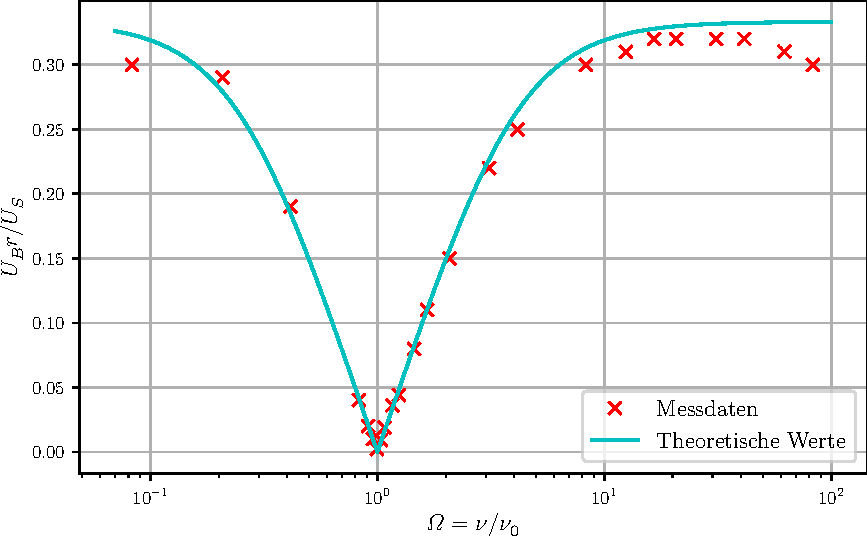
\includegraphics[width=\textwidth]{build/plot.pdf}
  \caption {Messwerte und Theoriekurven zur Bestimmung des Brewsterwinkels.}
  \label{fig:plot1}
\end{figure}

Außerdem werden Vergleichskurven geplottet. Hierfür werden die zuvor berechneten Mittelwerte der Brechungsindizes in die Fresnelschen
Formeln \eqref{eqn:senkrecht},\eqref{eqn:parallel} eingesetzt.

Aus dem Brewsterwinkel von $\alpha_B = \qty{75}{\degree}$ wird der Brechungsindex mithilfe von \autoref{eqn:brewster}
zu
\begin{align*}
  n_{\text{B}}&= 3.73 
\end{align*}
berechnet.







